	\documentclass[12pt,a4paper,ngerman]{article}
	
	\usepackage[utf8]{inputenc}
	\usepackage[T1]{fontenc}
	\usepackage{babel}
	\usepackage{graphicx} 
	\usepackage{hyperref} 
	%\usepackage[german]{algorithm2e}
	%\glqq \grqq{}
	\title{Vier-Gewinnt}
	\author{}
	
	\begin{document}
	\pagenumbering{gobble}
	\maketitle
	\newpage
	\tableofcontents
	\newpage
	\pagenumbering{arabic}
	\section{Einleitung}
	
	\section{Vier Gewinnt}
	\subsection{Spielidee}
	Die Grundidee des \glqq Vier Gewinnt\grqq{} Spieles ist es vier der eigenen Spielsteine bzw. Symbole in eine Reihe zu bringen.
	Dabei ist es egal ob dies horizontal, vertikal oder diagonal erreicht wird.
	Es spielen immer zwei Spieler gegeneinander, die abwechselnd einen Spielstein von oben in das Spielfeld einfügen, der dann so lange herunterfällt, bis er auf das Ende des Spielfeldes oder einen anderen Spielstein stößt.
	Sobald zum ersten Mal vier Spielsteine eines Spielers eine Reihe bilden, endet das Spiel und der betreffende Spieler gewinnt.
	Das Spielfeld in der Grundversion ist ein 7x6 Feld. Grundsätzlich sind aber auch größere und kleinere Felder möglich.
	\footnote{Lehmann, Jörg \glqq Vier gewinnt\grqq{} \url{http://www.brettspiele-report.de/vier-gewinnt/} Stand: 01.05.2019}
	\subsection{Implementation}
	Zunächst habe ich, wie in der Softwareentwicklung üblich die Klassendiagramme angelegt,\\
	\textit{Klassendiagramme}\\
	 um diese dann nach Umwandlung in ein Implementationsdiagramm dann umzusetzen.\\
	\textit{Implementationsdiagramme}\\
	Nach der Umsetzung versuchte ich die Laufzeit etwas zu senken, indem ich eine eigene Klasse erstellte an deren Objekten die Simulationen durchgeführt wird, um es mehr abzutrennen und um die redundante Speicherung der bisherigen Züge zu vermeiden.\\
	\textit{Klassendiagramme Vier Game und Logik}
	\section{Implementation der KI}
	\subsection{Taktik der KI}
	Die Taktik der KI (Künstliche Intelligenz) ist natürlich zu gewinnen oder eine (unmittelbare) Niederlage zu verhindern. Dazu wird ein Minimax-Algorithmus genutzt, um die beste Entscheidung zu treffen. Bei diesem Verfahren durchläuft der Algorithmus einen Suchbaum, der bei der maximalen Suchtiefe jedem Ergebnis einen Wert zuweist oder, wenn schon vorher ein Sieg oder eine Niederlage auftritt, diesen jeweils einen positiven bzw. negativen Wert zuordnet. Bei der Auswertung wird dann immer das Minimum der gegnerischen Züge gewertet und das Maximum der eigenen, so dass jeder Spieler ein \glqq perfektes \grqq{} Spiel spielt. Des Weiteren bevorzugt der Algorithmus einen schnellen Sieg bzw. eine spätere Niederlage.
		\\
	Neben dem Minimax-Algorithmus könnte man auch vorberechnete Eröffnungszüge nutzen, aber diese unterscheiden sich für jede Spielfeldgröße. Einige Spiele gelten dadurch auch schon als gelöst:
	\begin{figure}
		\centering
		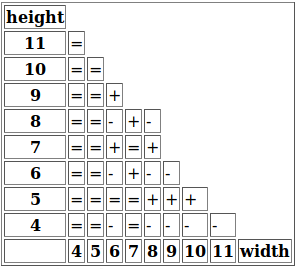
\includegraphics[width=0.7\linewidth]{w-h-viergew}
		\caption{}
		\label{fig:w-h-viergew}
		\footnote{Tromp, John  \glqq John's Connect Four Playground \grqq{} \url{http://tromp.github.io/c4/c4.html} Stand: 01.05.2019}
	\end{figure}
    \newpage
	Zu Abbildung 1:\\
	+ der 1. Spieler gewinnt\\
	- der 2. Spieler gewinnt\\
	= Unentschieden\\
	
	
	
	\subsection{Schwächen}
	Theoretisch sind der KI nur Grenzen gesetzt durch die Rechenleistung bzw. die Tiefe der Simulation
	\subsection{Effizienzbetrachtung}
	Um mehr Züge zu simulieren ist erheblich mehr Rechenleistung erforderlich. Die Komplexität steigt nahezu exponentiell, aber je weiter das Spiel fortgeschritten ist und je weniger Möglichkeiten es gibt, desto schneller wird der Algorithmus. Ich habe Simulationen durchgeführt mit verschiedenen Feldgrößen und habe den ersten Zug von der KI berechnen lassen, dabei habe ich die Zeit gemessen und damit passende Tiefen gewählt, um die Zeit bei weniger als 10 Sekunden zu halten. Hätte ich die vordefinierten Pfade genommen, wäre deutlich an Rechenzeit gespart worden, jedoch bräuchte man zum Erstellen dieser sehr lange bzw. würde es den Rahmen dieser Facharbeit sprengen. Auch wäre es möglich anstatt der VierLogik Klasse auch einfach nur kopierte Arrays zu verwenden, aber dabei ist es schwer darauf zu achten, dass keines dieser Arrays verändert wird.\\
	Aber nun zur Effizienz bei verschiedenen Feldgrößen. Da die Höhe nicht so ausschlaggebend ist wird hier nur betrachtet wie sich die Ausführungszeit verändert, wenn die Suchtiefe und die Feldbreite variiert werden. Die KI versucht in jedem Fall den ersten Zug zu berechnen.
	\textit{Diagramm 5-7-9w 1-10d}
	\section{Künstliche Intelligenz}
	\textit{Definition}
	\subsection{Aktueller Stand}
	\textit{tensorflow,machine learning}
	\subsection{Ausblick}
	\textit{Filme usw. (Wargames,Terminator,2001,I Robot)}
	
\end{document}

